\documentclass[9pt, compress, xcolor=table]{beamer}


\usetheme{m}

\usepackage{amsmath,amssymb}
\usepackage{booktabs}
\usepackage[scale=2]{ccicons}
\usepackage{minted}
% \usepackage[utf8]{inputenc}
% \usepackage[T2A]{fontenc}
% \usepackage[english, russian]{babel}
%%% For accessing system, OTF and TTF fonts
%%% (would have been loaded by polylossia anyway)
\usepackage{fontspec}
%%% For language switching -- like babel, but for xelatex
\usepackage{polyglossia}
\setmainfont{PT Sans} % вообще шрифты определяются в теме бимера
\setmainlanguage{russian}
\setotherlanguages{english} %% or other languages

\usepackage{graphicx}
\usepackage{tabu} % https://ru.sharelatex.com/learn/Tables
\DeclareGraphicsExtensions{.pdf,.jpg,.png}
\graphicspath{{../images/}{./images/}}

\colorlet{Mycolor1}{green!50!blue!50!}

\usemintedstyle{trac}

\title{Физические принципы микроскопии сверхвысокого разрешения}
\subtitle{осенний семестр, 2018}
\author{ассистент, к.ф.-м.н. Шутова О.А.}
\institute{МГУ им. М.В. Ломоносова, физический факультет}

\begin{document}

\maketitle

\plain{}{Лекция 4. Бижнепольная микроскопия: обзор методов}

\begin{frame}{Идея лекции}


\begin{columns}[c]
\column{6.5cm}
\begin{center}
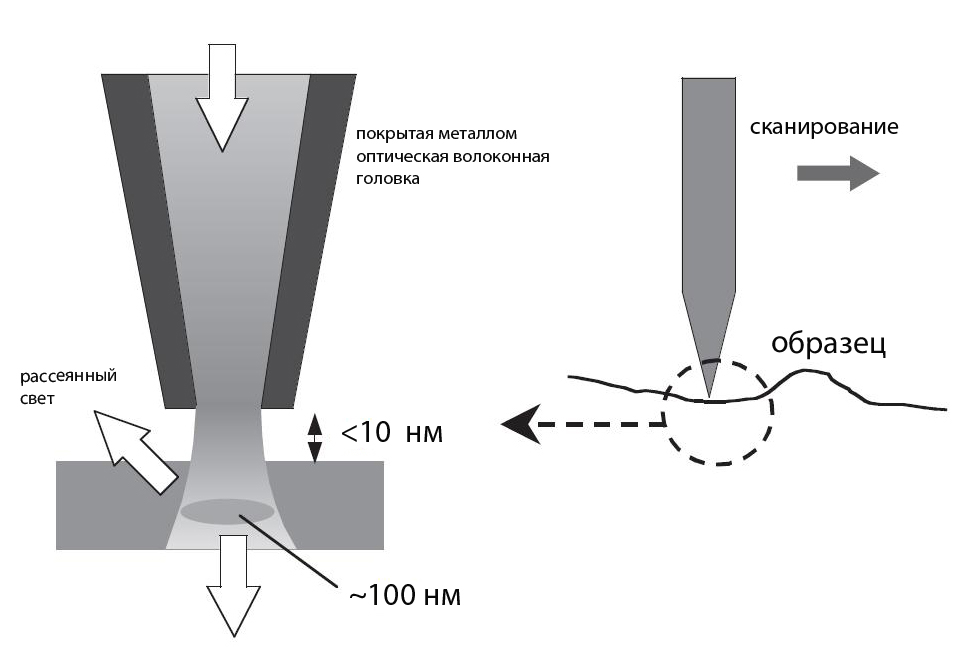
\includegraphics[width=0.9\textwidth]{nfm2}
\\* с апертурным зондом \textcolor{blue}{c-SNOM}
\end{center}



\column{6.5cm}
\begin{center}
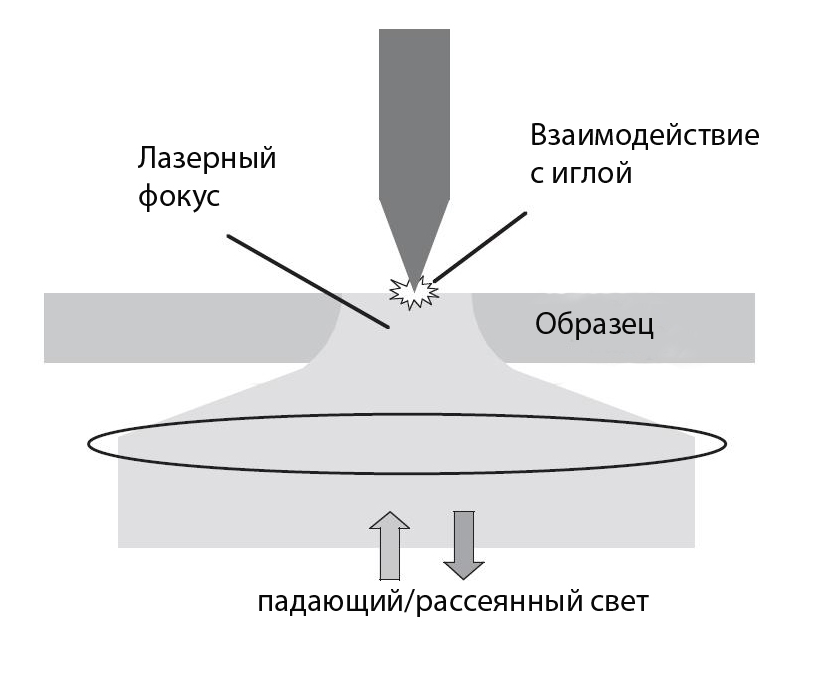
\includegraphics[width=0.9\textwidth]{nfm3}
\\*с безапертурным зондом \textcolor{blue}{s-SNOM} (может быть как диэлектрическим, так и металлическим)
\end{center}

\end{columns}

Различие методов обусловливается главным образом характером \textcolor{red}{взаимодействия между зондом и образцом}, обусловленного физическим законом, который используется для его усиления и запирания.

\end{frame}

\begin{frame}{Полезные аббревиатуры}

\colorbox{yellow!30}{\textcolor{red}{c-SNOM} (collecting scanning near-field optical microscope) - микроскопия} \newline \colorbox{yellow!30}{с апертурным зондом}

\colorbox{yellow!30}{\textcolor{red}{s-SNOM} (scattering scanning near-field optical microscope) - микроскопия} \\* \colorbox{yellow!30}{с безапертурным зондом}

\textcolor{red}{PSTM} (photon scanning tunelling microscopy) - на основе создания условий нарушенного полного внутреннего отражения 

\textcolor{red}{SIAM} (scanning interferometric apertureless microscopy) - модуляционная методика, схожая с методом временной метки для дискретных событий

\textcolor{red}{FRET} (F\"orster resonance energy transfer) - микроскопия на основе безызлучательного механизма переноса энергии по Фёрстеру

\textcolor{red}{TERS/SERS} (tip/surface enhanced Raman scattering)
- на основе усиленного зондом/поверхностью рамановского рассеяния

\textcolor{red}{SPP-SNOM} - подложка или зонд покрывается фотонным материалом и усиление поля достигается за счет возбуждения ППП

\textcolor{red}{SHG-SNOM} - следим за ближнепольным сигналом второй оптической гармоники (не путать с модуляционными техниками!!!)


\end{frame}

\begin{frame}{Различные зонды ближнепольной оптической микроскопии}
    \begin{center}
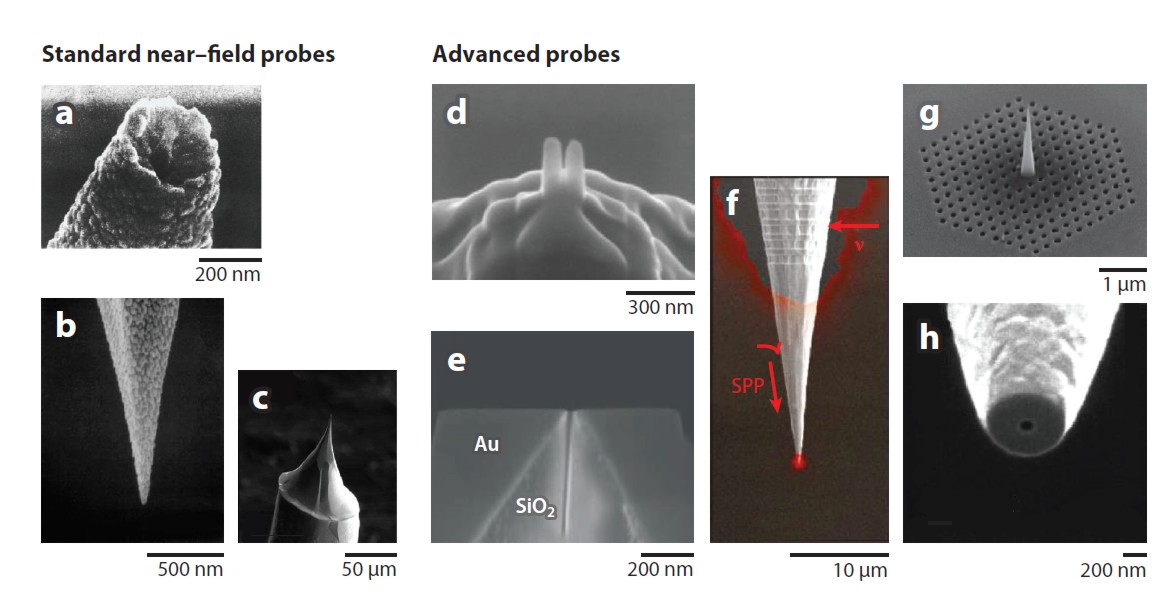
\includegraphics[width=0.9\textwidth]{probes}
\newline Схема PSTM
\end{center}

R.J.Hermann, M.J.Gordon "Nanoscale optical microscopy and spectroscopy using near-field probes". Annual Reviews.2018.
\end{frame}

\plain{}{PSTM - photon scatterring tunnelling microscopy}

\begin{frame}{Общая схема метода}

\begin{columns}[c]
\column{6.5cm}
\begin{center}
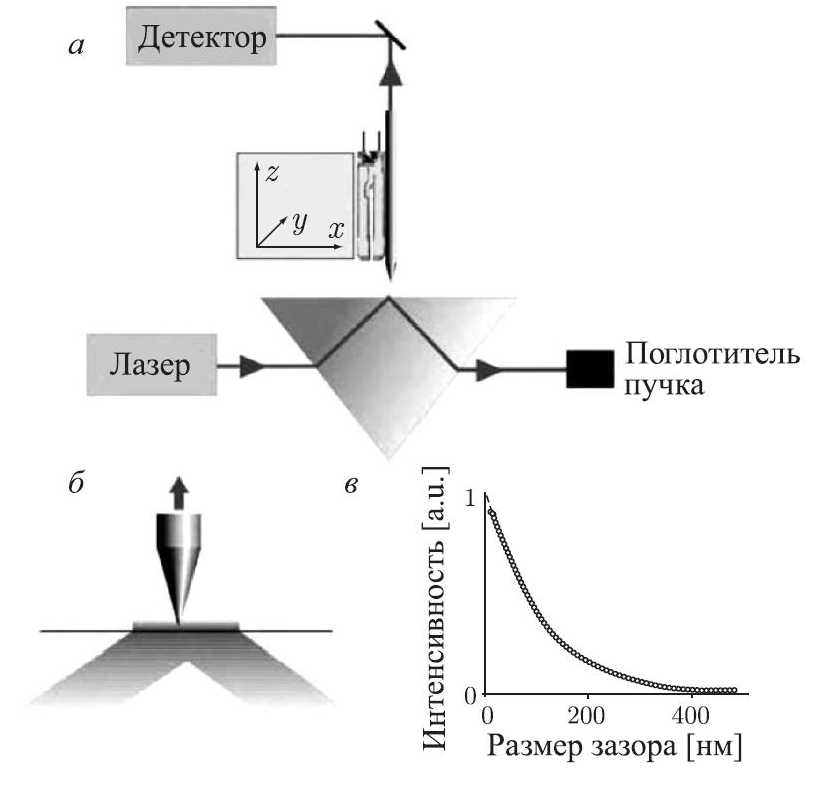
\includegraphics[width=0.9\textwidth]{nfm17}
\newline Схема PSTM
\end{center}




\column{6cm}
\begin{itemize}
\item \textcolor{red}{Преимущество} в малом возмущении поля исследуемого объекта
\item \textcolor{blue}{Недостаток} в малом пространственном запирании поля
\item \textcolor{blue}{Недостаток} в попадании засветки в зонд через боковые поверхности
\item При условии совмещения со схемой гетеродинирования можно достичь разрешающей способности в сотни нанометров
\item \textcolor{blue}{Недостаток} в сложной калибровке: вариативность формы зонда, зав-ть от объекта
\end{itemize}
\end{columns}
В группе методов относится к c-SNOM.

\end{frame}

\begin{frame}{Возможности PSTM}
\begin{columns}[c]
\column{6.5cm}
\begin{center}
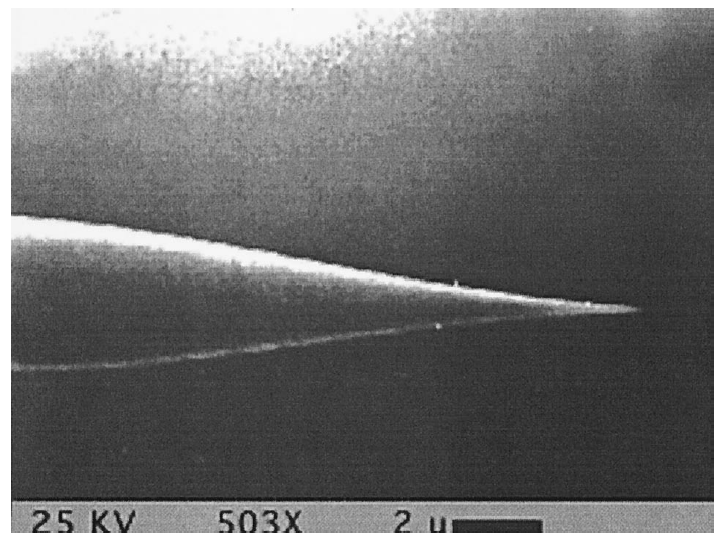
\includegraphics[width=0.9\textwidth]{nfm30}
\newline Изображение зонда для  PSTM, полученного методом травления кончика оптического волокна
\end{center}

\column{6.5cm}
\begin{center}
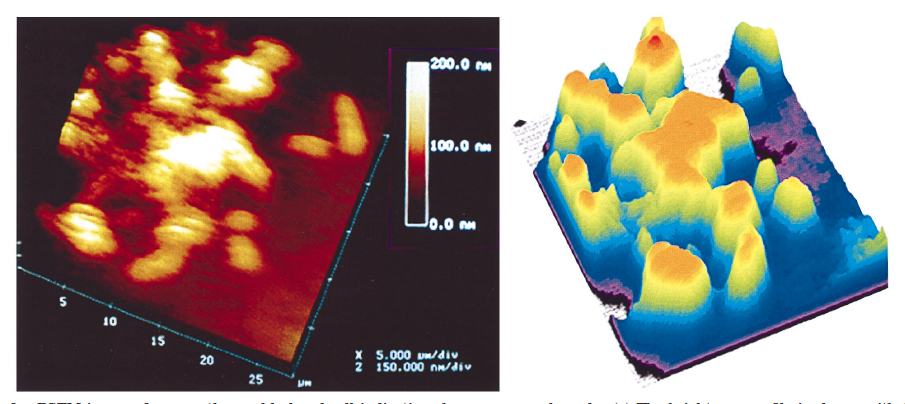
\includegraphics[width=0.9\textwidth]{nfm31}
\newline Изображение клетки тела человека, в процессе ее лизирования, видно, как выступают хромосомы. \\*\colorbox{yellow!30}{\small{F.Meriaudeau et al. Applied Optics. v.37, n.31, 1998.}}
\end{center}

\end{columns}

Для получения адекватного разрешения и отношения сигнала к шуму, если мы хотим исследовать объект как он есть, без использования подкрашивающих растворов, необходимо укорачивать длину волны и дополнять информацию спектроскопическими исследованиями. Все это делает методику довольно сложной.

\end{frame}

\begin{frame}{Возможности PSTM}
\begin{columns}[c]
\column{6.5cm}
\begin{center}
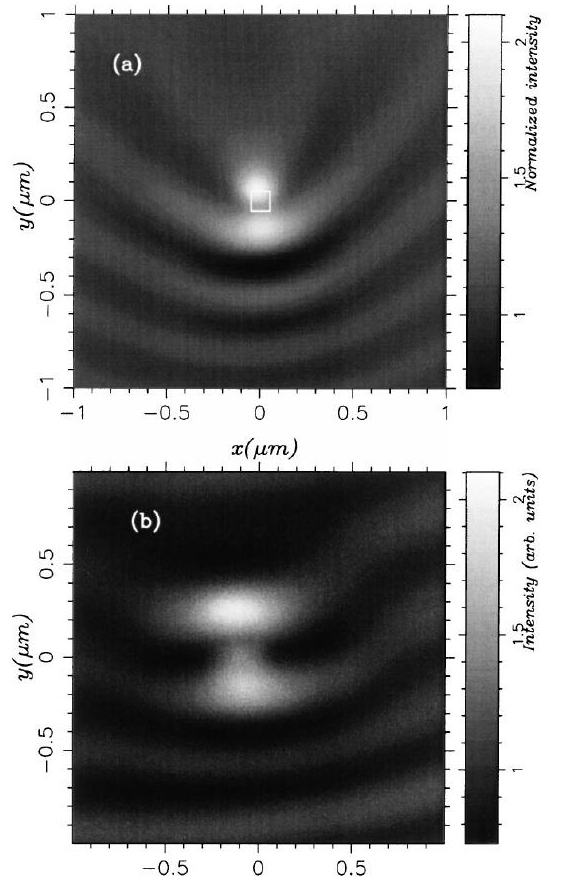
\includegraphics[width=0.7\textwidth]{nfm18}
\newline Изображение золотого квадратика размером $100*100*40 \text{нм}^3$, зазор менее 45 нм.
\end{center}

\column{6.5cm}
\begin{center}
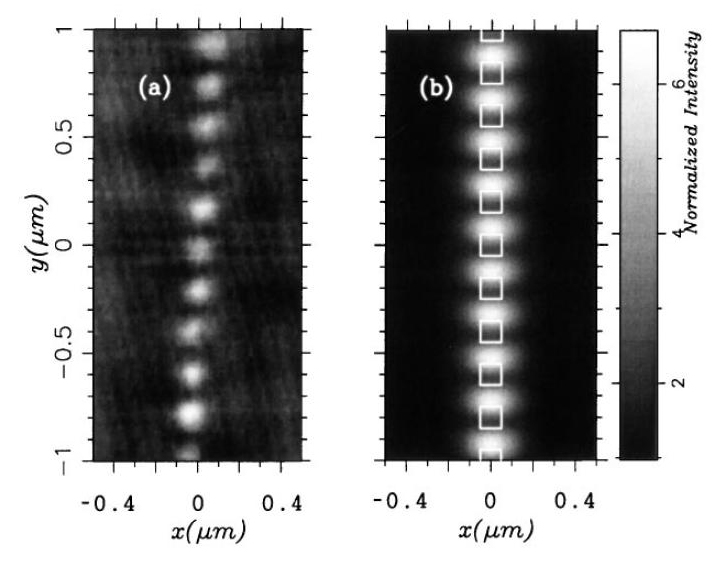
\includegraphics[width=0.95\textwidth]{nfm16}
\newline Много таких квадратиков, разделенных расстоянием 100 нм. Видим как концентрируется поле за счет коллективных эффектов. \\*\colorbox{yellow!30}{\small{J.R.Krenn et al. Phys.Rev.Lett. v.82 1999.}}
\end{center}

\end{columns}

\end{frame}

\plain{}{SIAM -scanning interferometric apertureless microscopy}

\begin{frame}{Основы метода}
\begin{columns}[c]
\column{6.5cm}
\begin{center}
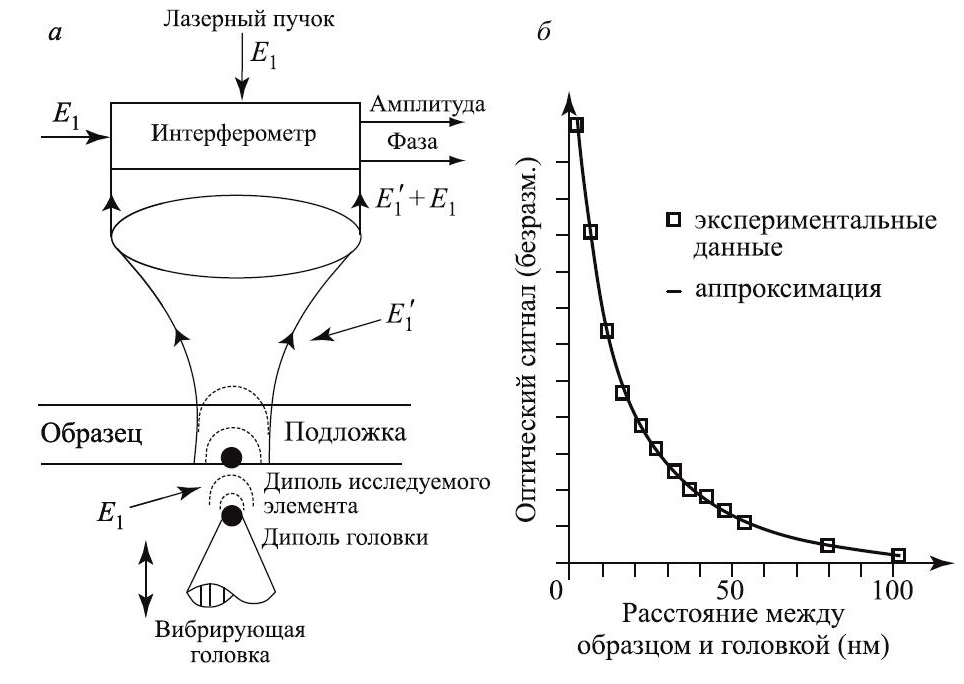
\includegraphics[width=0.9\textwidth]{nfm14}
\newline Возможная схема в модуляционной технике микроскопии на рассеяния
\end{center}

\column{6cm}
\begin{itemize}
\item Как правило это металлический безапертурный зонд, позволяющий лучше усилить и сконцентрировать поле
\item Зонд вибрирует на определенной частоте
\item Сигнал демодулируется на гармониках частоты модуляции
\item Благодаря технике модуляции можно изучать фазу ближнего поля
\item Разрешающая способность может достигать 10 нм
\end{itemize}

\end{columns}
В группе методов относится к \textcolor{blue}{s-SNOM}.

\small{F. Keilmann, R.Hillenbrand "Near-field microscopy by elastic light scattering from a tip". Philosophical Transactions A R.Soc.Lond. 2004.
\\*
P. Royer et al. "Near-field optical patterning and structuring based on local-field enhancement at the extremity of a metal tip". Philosophical Transactions A R.Soc.Lond. 2004.}
\end{frame}

\begin{frame}{Сравнение металлического и диэлектрического зонда}
\begin{columns}[c]
\column{6.5cm}
\begin{center}
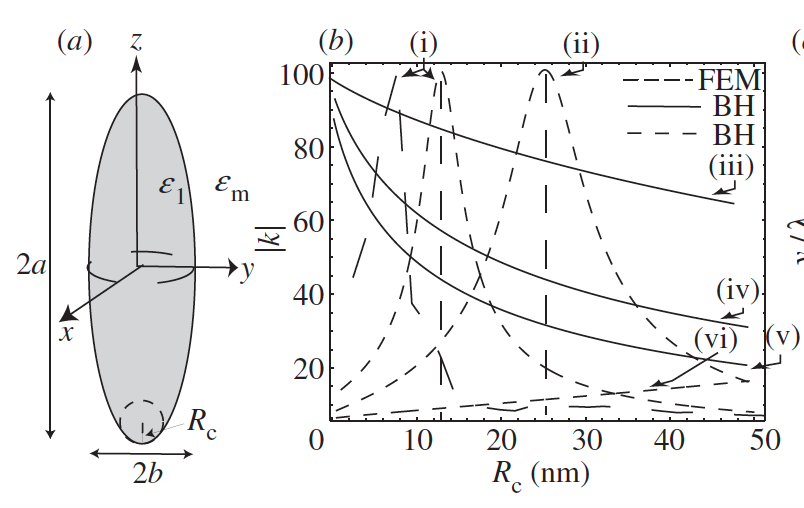
\includegraphics[width=0.9\textwidth]{nfm32}
\newline Усиление поля ($|k|=|E(\xi=0)|/|E_0|$) в модели эллипсоида. Сплошные кривые - диэлектрик ($\epsilon =10.9824+1.3280 \imath$), пунктирные - металл $\epsilon =-10.9824+1.3280 \imath$ по модели Борена-Хафмен \\*
См. книгу: К. Ф. Борен, Д. Р. Хафмен. Поглощение и рассеяние света малыми частицами. Пер. с англ. З. И. Фейзулина и др., предисл. В. И. Татарского. - М. : Мир, 1986.
\end{center}

\column{6.5cm}
\begin{center}
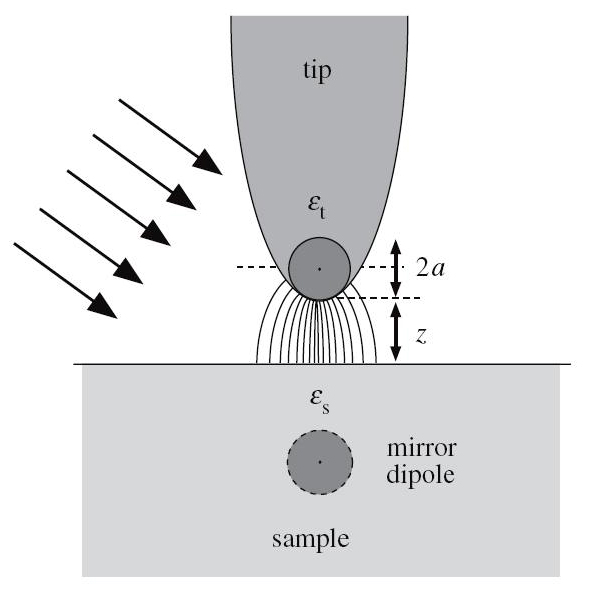
\includegraphics[width=0.95\textwidth]{nfm5}
\newline В квазистатическом пределе с учетом малости кончика зонда по сравнению с длиной волны можно пользоваться методом изображений.
\end{center}

\end{columns}

\end{frame}

\begin{frame}{Основа метода}
\begin{columns}[c]
\column{6.5cm}
\begin{center}
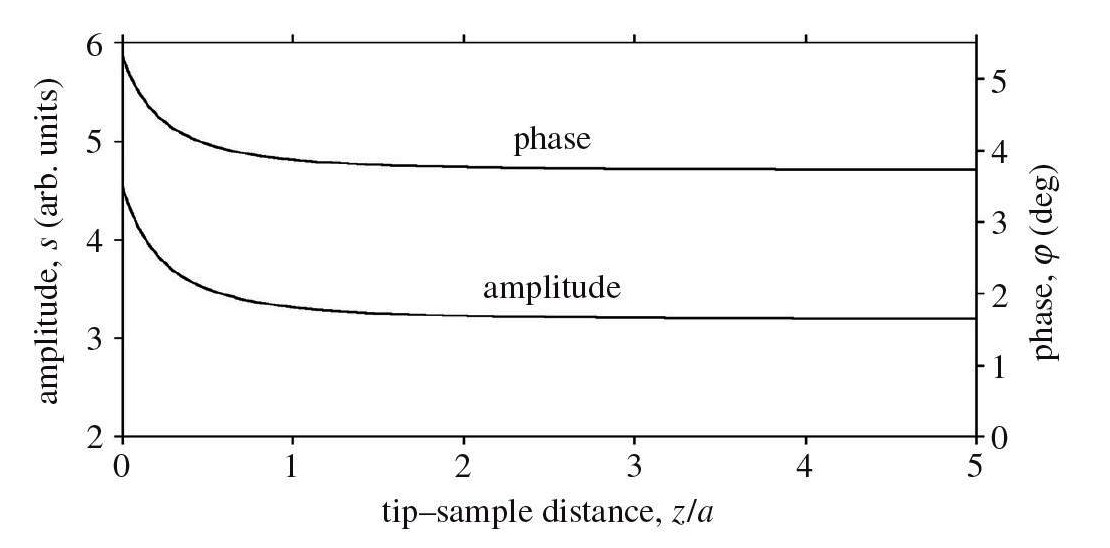
\includegraphics[width=0.9\textwidth]{nfm6}
\\* если мы представим $\alpha_{eff} = s e^{\imath \phi}$, то соответствующие амплитуда и фаза будут монотонно спадать по мере удаления от образца
\end{center}

\column{6.5cm}
\begin{center}
Эффективная поляризуемость системы "зонд+образец"
\begin{equation*}
\alpha_{eff}=\frac{\alpha(1+\beta)}{1-\alpha\beta/(16\pi(\alpha+z)^3)},
\end{equation*}
где $\alpha$ и $\beta$ выражаются через восприимчивости зонда и образца $\epsilon_t$  и $\epsilon_s$
\begin{equation*}
\alpha=4\pi a^3\frac{\epsilon_t-1}{\epsilon_t+2}
\end{equation*}
\begin{equation*}
\beta=\frac{\epsilon_s-1}{\epsilon_s+1}
\end{equation*}
\end{center}
\end{columns}

\begin{center}
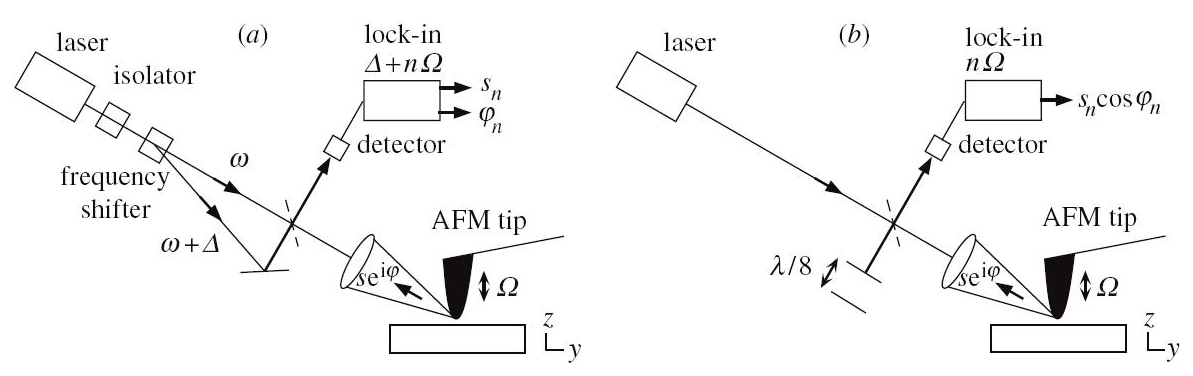
\includegraphics[width=0.9\textwidth]{nfm8}
\end{center}

\end{frame}

\begin{frame}{Зависимость усиления от поляризации}
\begin{columns}[c]
\column{8.5cm}
\begin{center}
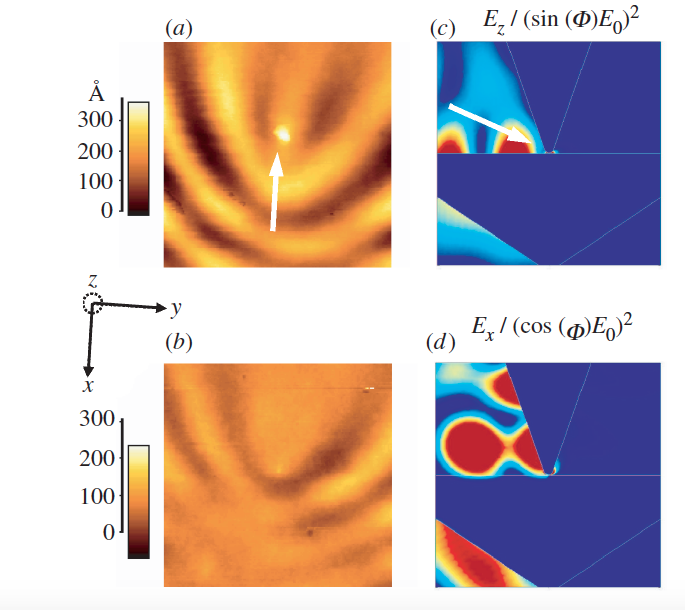
\includegraphics[width=0.9\textwidth]{nfm33}
\\* 
\end{center}

\column{4cm}

Диэлектрический зонд, покрытый кобальтом, с кривизной около 20 нм. Верхний ряд - поляризация направлена вдоль зонда (перпендикулярно экрану), нижний ряд - вдоль s-поляризация 

\end{columns}

\end{frame}

\begin{frame}{Вырезать засветку: техника модуляции}

\begin{center}
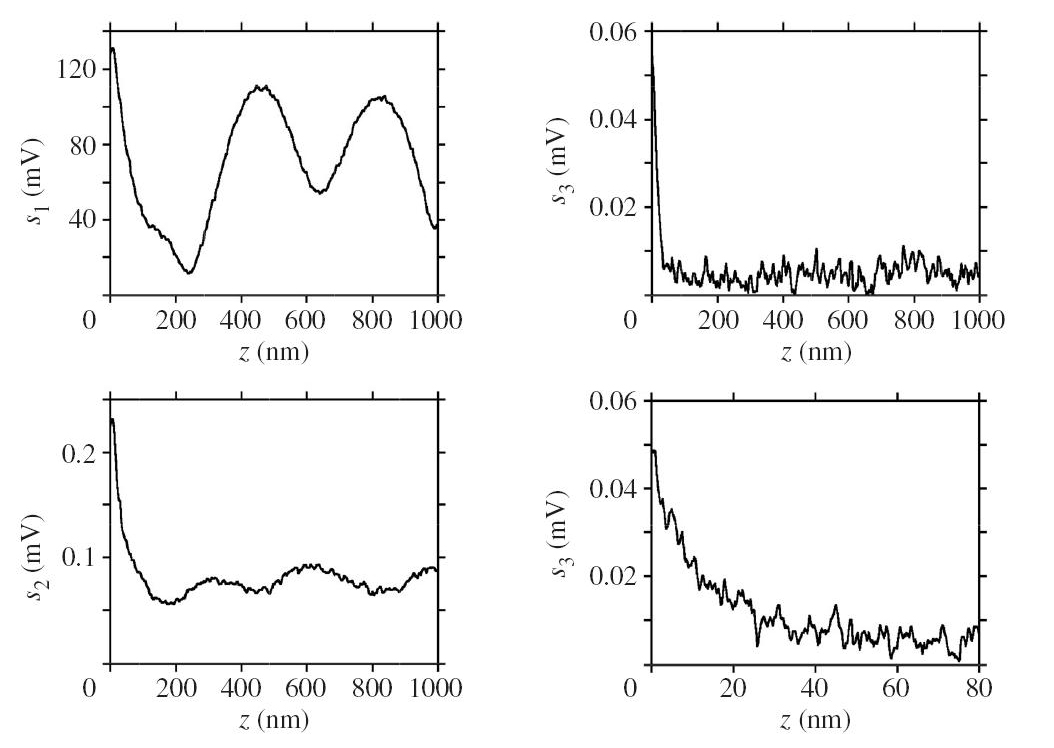
\includegraphics[width=0.85\textwidth]{nfm7}
\\* Зонд изготовлен из платины, образец - кремний, радиус кривизны 20 нм, амплтуда модуляции 20 нм, длина волны излучения 633 нм. Демодуляция на высокий гармониках позволяет оставить лишь сигнал ближнего поля (4-ый график - увеличение 3-го). 
\end{center}

\end{frame}

\begin{frame}{Чувствительность к веществу подложки}

\begin{center}
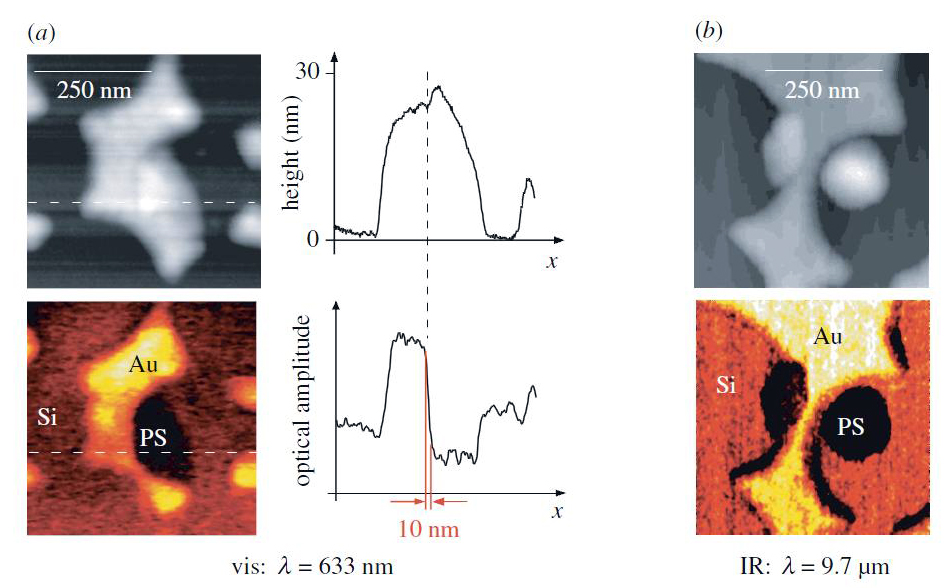
\includegraphics[width=0.9\textwidth]{nfm10}
\\* 
Благодаря тому, что эффективная поляризуемость зависит также и от вещества образца, данный метод обладает хорошим контрастом при изменении этих свойств (своего рода "оптическое подкрашивание"): конгломерат металл-диэлектрик-полупроводник.
\end{center}

\end{frame}

\begin{frame}{Чувствительность к плазмонному резонансу}

\begin{center}
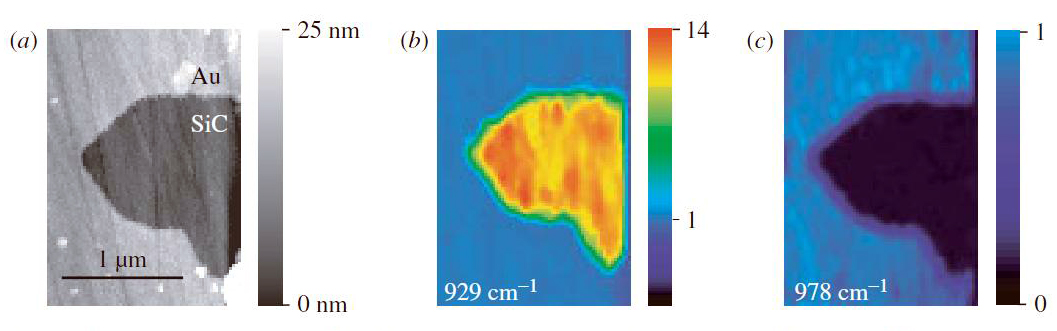
\includegraphics[width=0.9\textwidth]{nfm12}
\\* Настройка на плазмонный резонанс золотой
\\*
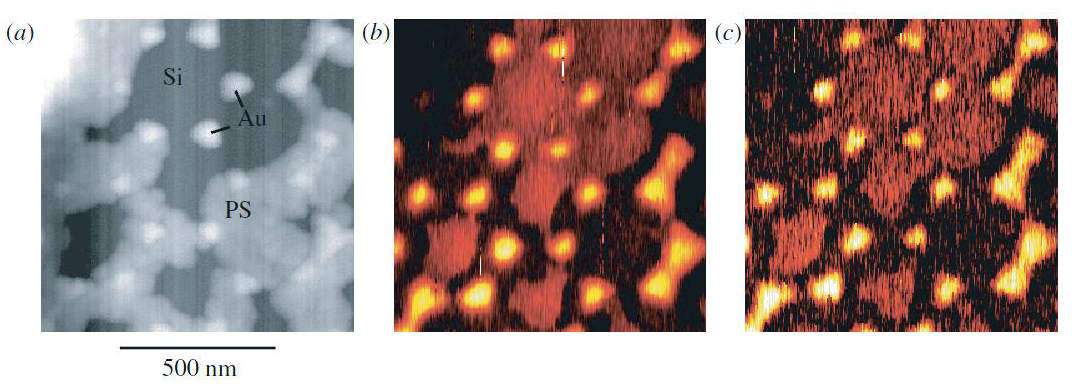
\includegraphics[width=0.9\textwidth]{nfm11}
\\* Сравнение 3-й и 4-1 гармоник демодуляции.
\end{center}

\end{frame}

\begin{frame}{Локализация отклика}
\begin{columns}[c]
\column{6.5cm}
\begin{center}
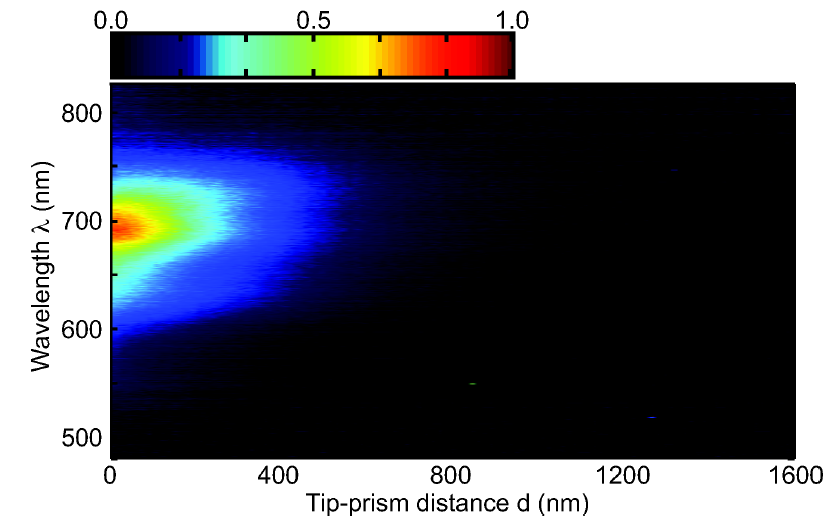
\includegraphics[width=0.9\textwidth]{plasmon-res}
\\* \small{То что "лепесток" вытянут строго горизонтально говорит нам об отсутствии спектрального сдвига по мере приближения к поверхности}
\end{center}

\column{6.5cm}
\begin{center}
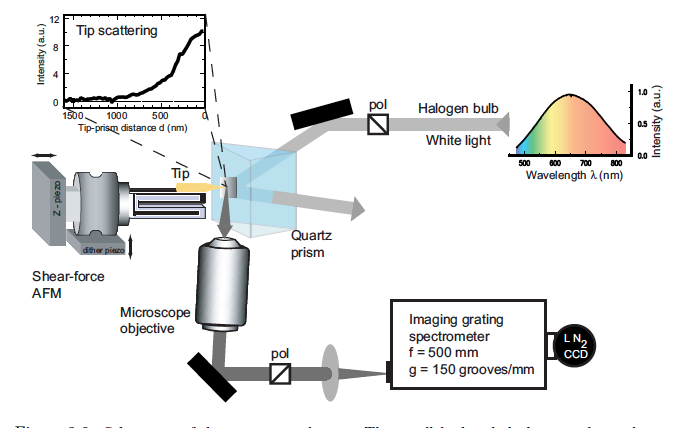
\includegraphics[width=0.9\textwidth]{exp_plasm_res}
\\* 
\end{center}
\end{columns}
\begin{center}


\end{center}

В случае если бы имели место эффекты макроскопического движения зарядов по объему зонда, при приближении к поверхности мы бы имели постепенное изменение пространственного распределения зарядов. Это неизбежно приводило бы к сдвигу спектральной частоты отклика, т.к. эта частота определяется в т.ч. форм-фактором и величиной этого распределения.

\end{frame}

\begin{frame}{Влияние форм-фактора и вещества зонда }
\begin{columns}[c]
\column{6.5cm}
\begin{center}
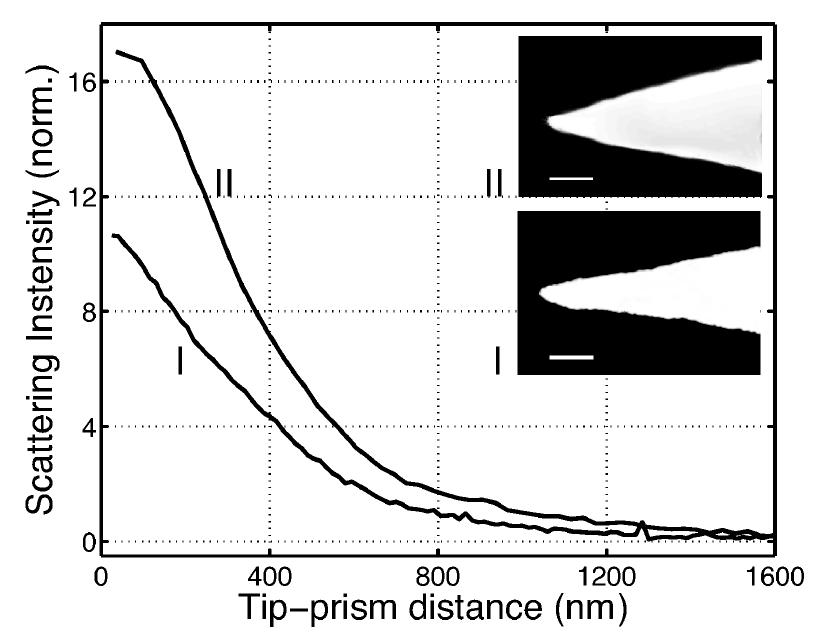
\includegraphics[width=0.8\textwidth]{optant_18}
\\* Более широкий зонд дает меньшее усиление
\end{center}

\column{6.5cm}
\begin{center}
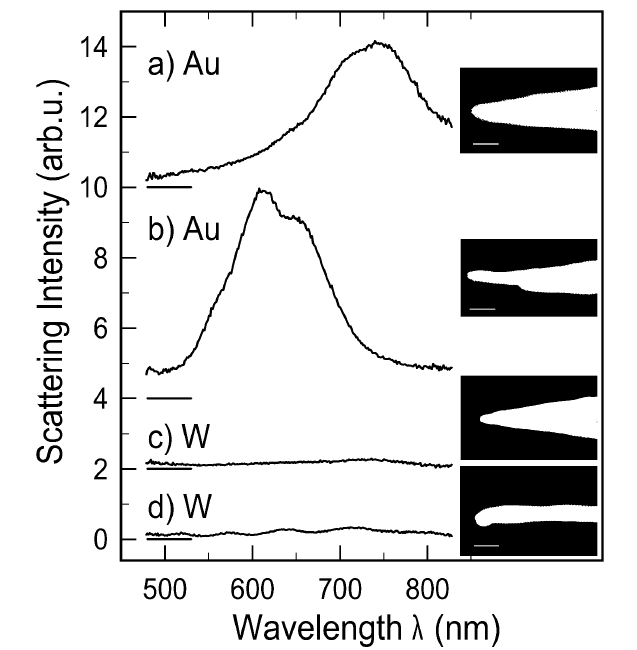
\includegraphics[width=0.9\textwidth]{optant_19}
\\* Вольфрам, хотя и металл, но в видимом диапазоне $\epsilon_W\approx5+\imath 19$, плазмонного резонанса нет.
\end{center}
\end{columns}

\end{frame}


\begin{frame}{Введение голографического метода}

R. Hillenbrand. Nature. 2014.
\begin{center}
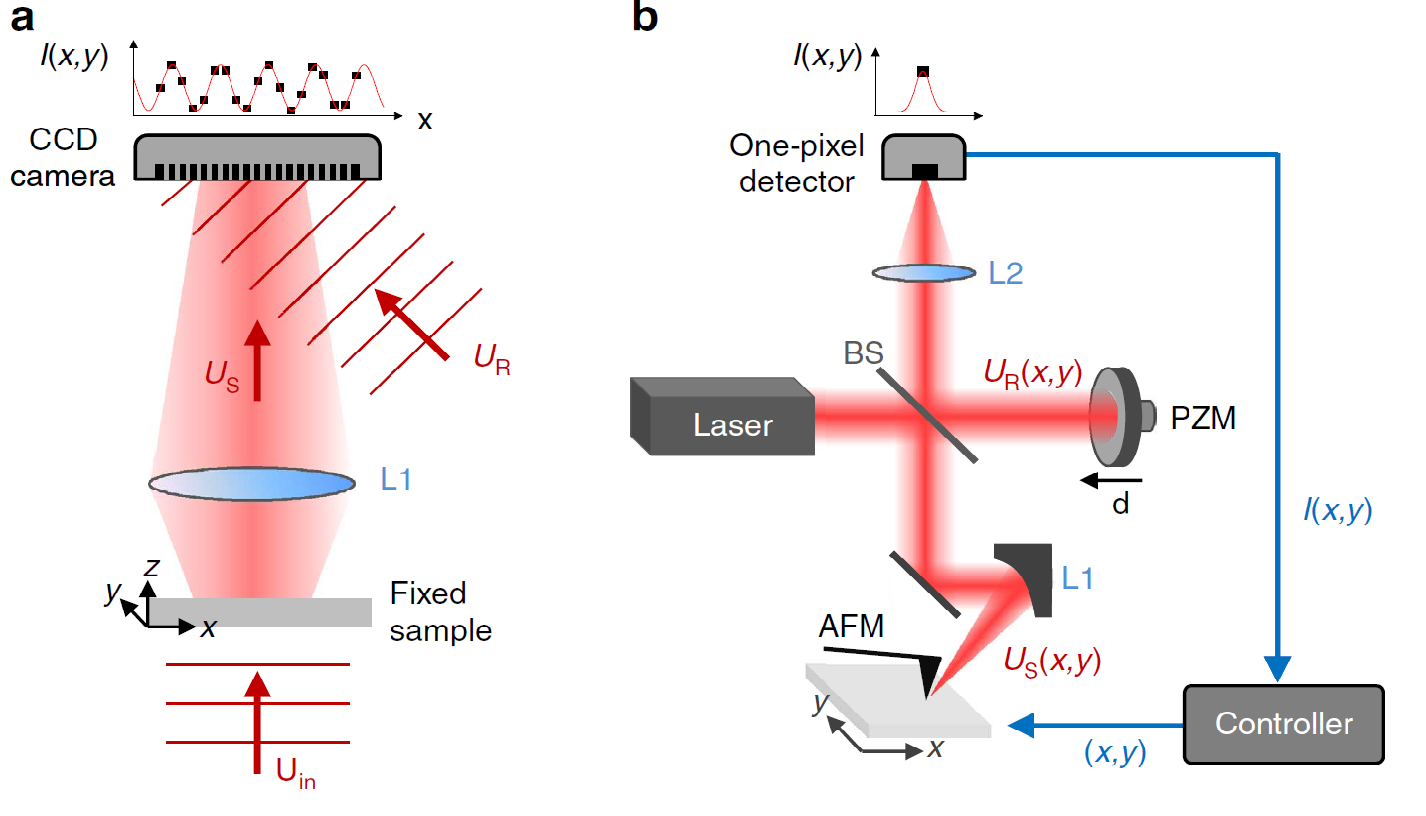
\includegraphics[width=0.8\textwidth]{hillen_1}

Схема во многом похожа на схему классической голографии (слева) за тем лишь исключением, что опорный пучок в каждой точке имеет уникальную фазу, получаемую в результате движения пьезоактивируемого зеркала (PZM) с определенной скоростью.

\end{center}
\end{frame}

\begin{frame}{Верификация работы на примере визуализации ИК-антенны}

\begin{center}
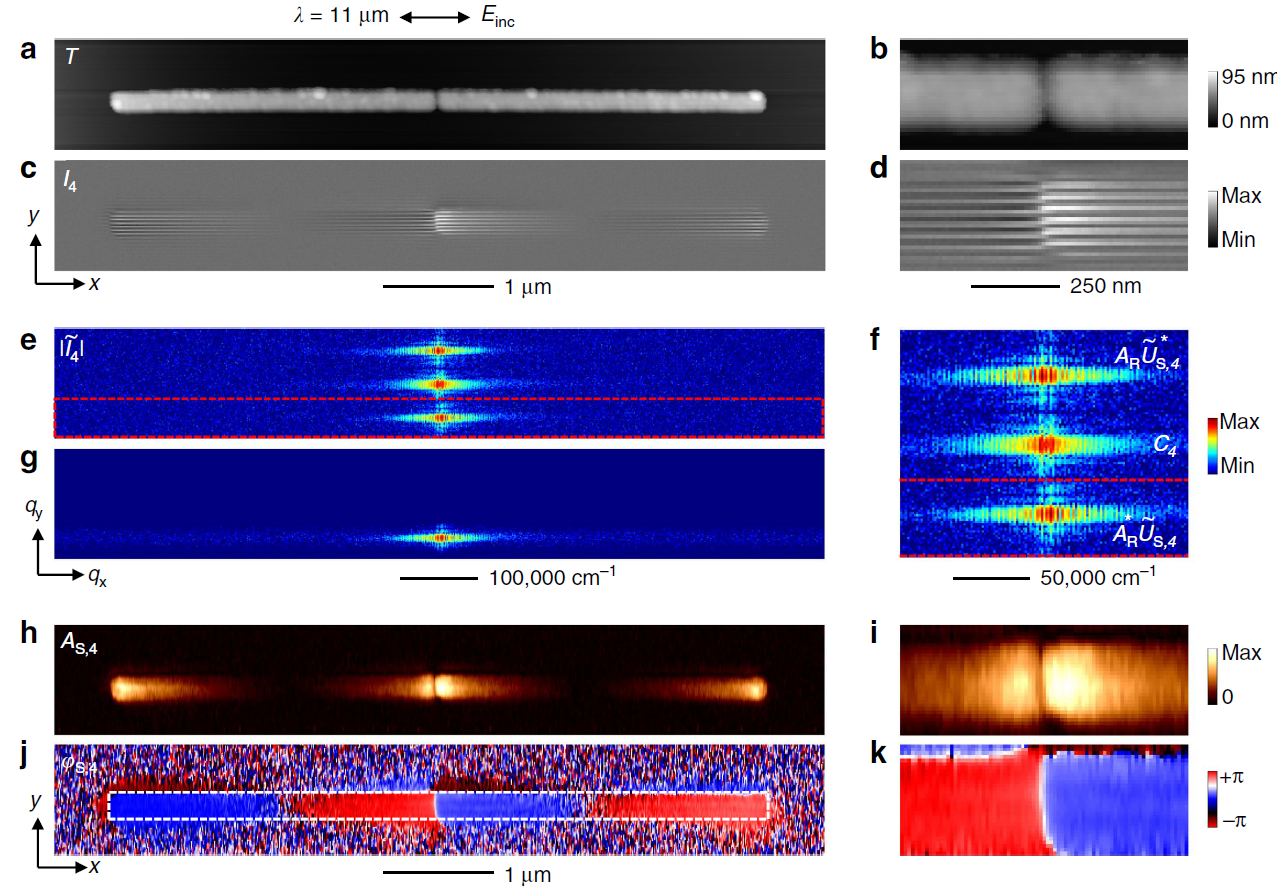
\includegraphics[width=0.75\textwidth]{hillen_2}
\begin{equation*}
    \varphi_R (\vec r) = \frac{2\pi}{\lambda}2d(\vec r)=\vec k_{||}\cdot \vec r
\end{equation*}
\begin{equation*}
    \hat I_n (\vec q) = C_n (\vec q)+A_R \hat U^*_{S,n}(\vec k_{||}-\vec q)+A_R^* \hat U_{S,n}(\vec k_{||}+\vec q)
\end{equation*}

$ C_n (\vec q)$ - автокорреляционное слагаемое, содержащее мультипликативный шум

\end{center}
\end{frame}

\begin{frame}{Одновременное измерение амплитуды и фазы}

\begin{center}
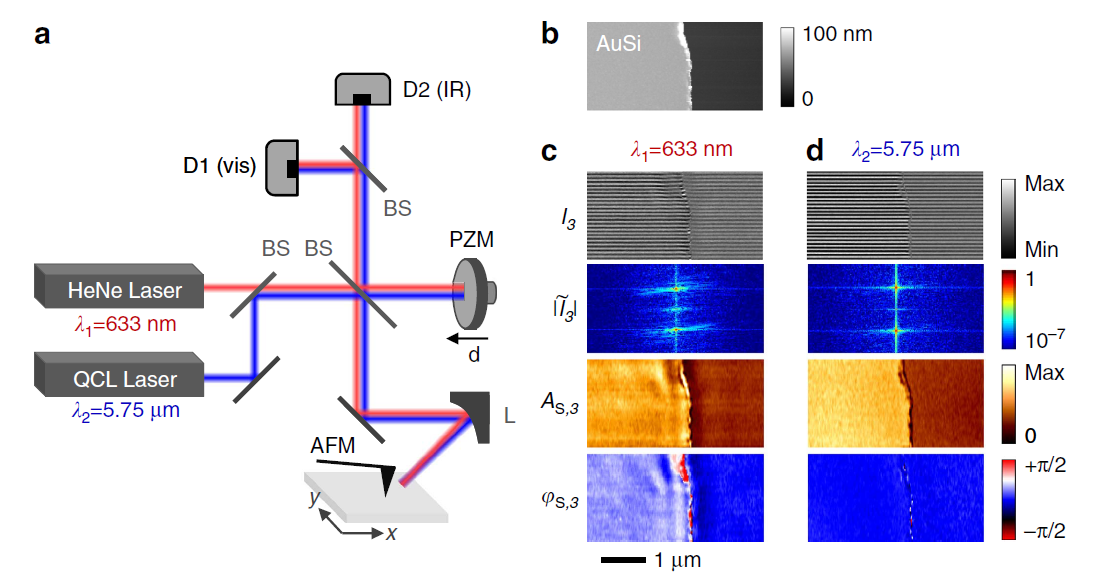
\includegraphics[width=0.95\textwidth]{hillen_3}

Край золота на кремнии.

$\lambda_1=5.75$ микрон
$\lambda_2=633$ нанометра

Отсутствие фазового контраста для ИК указывает нам на то, что не возбудился плазмонный резонанс.
\end{center}
\end{frame}

\begin{frame}{Визуализация графена-I}

\begin{center}
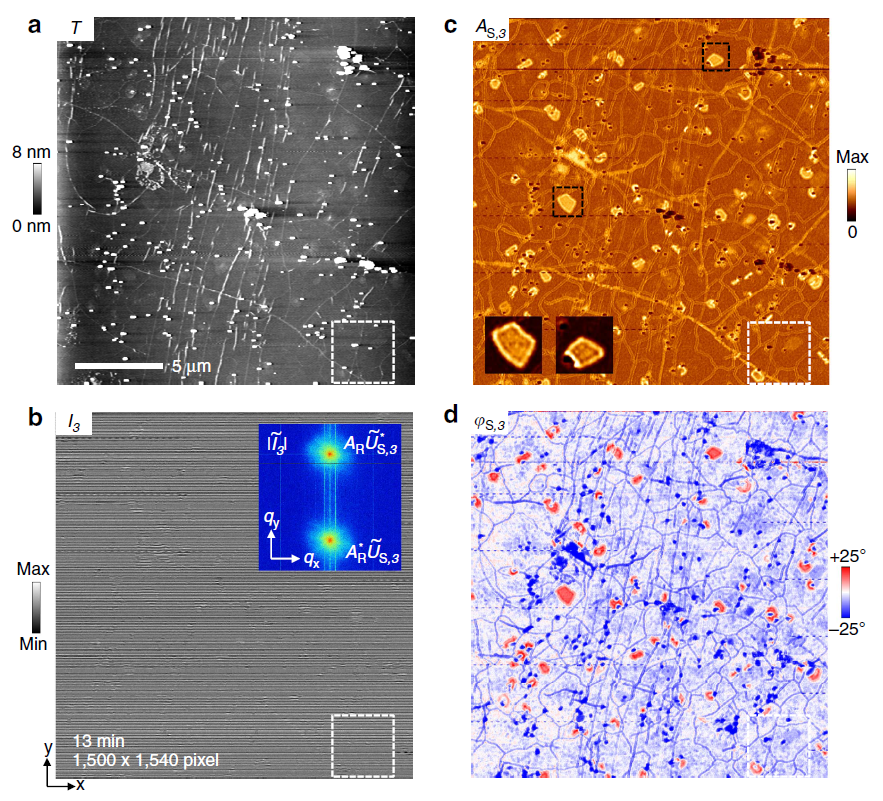
\includegraphics[width=0.8\textwidth]{hillen_4}

\end{center}
\end{frame}

\begin{frame}{Визуализация графена-II}

\begin{center}
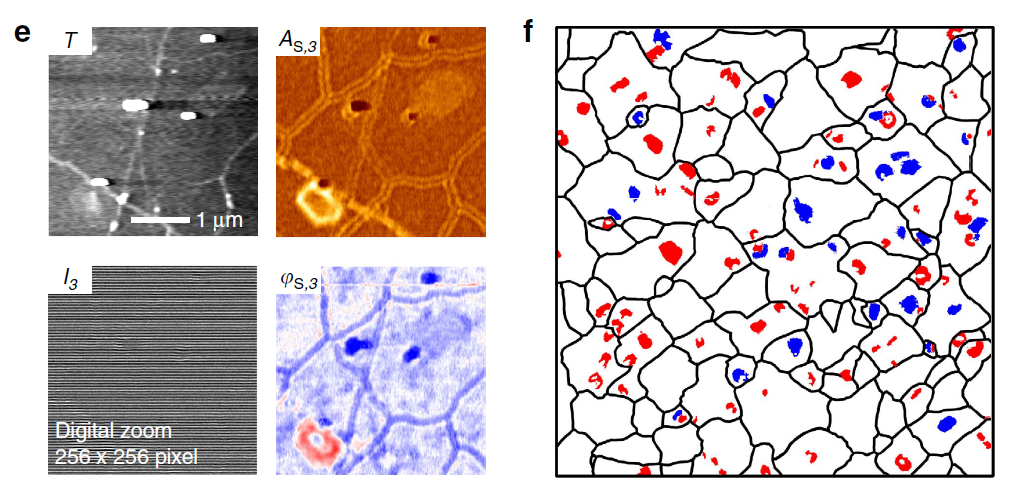
\includegraphics[width=0.97\textwidth]{hillen_5}

Исследовался образец графена, полученного методом химического осаждения паров (CVD), размером $21\times21 \text{микрон}^2$.

\end{center}
\end{frame}

\begin{frame}{Сравнение методов}
Сравнение гомодинного, гетеродинного, псевдогетеродинного и голографического метода (SOH) анализа отраженного сигнала.
\begin{center}
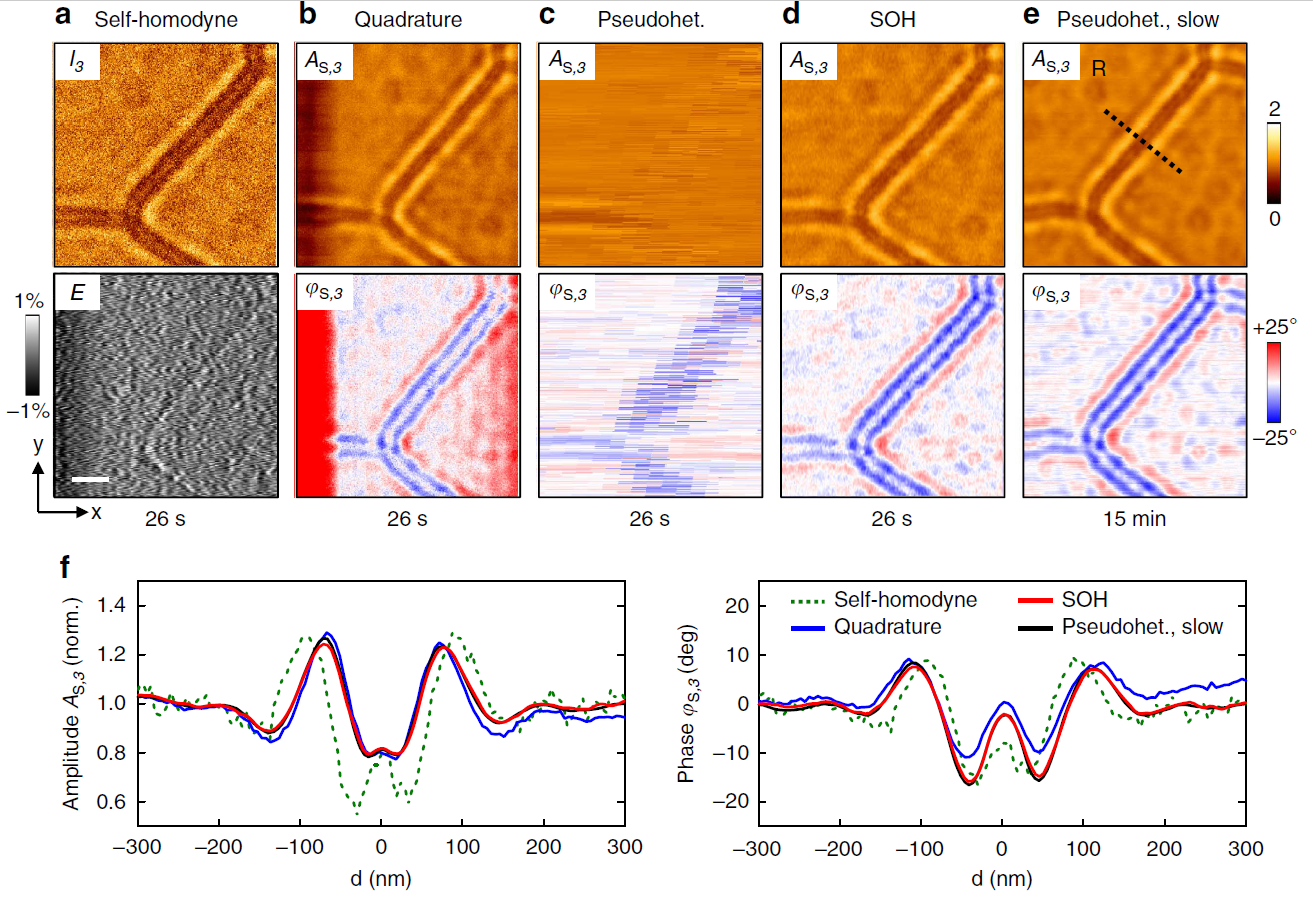
\includegraphics[width=0.9\textwidth]{hillen_6}
\small{2.3 мегапискеля в SOH поучено за 14 мин, коммерческий псевдогетородинный (справа) - 8 часов.}

\end{center}
\end{frame}

\plain{}{FRET - F\"orster resonance energy transfer microscopy}

\begin{frame}{Фёрстеровский перенос энергии}
\begin{columns}[c]
\column{7cm}
\begin{center}
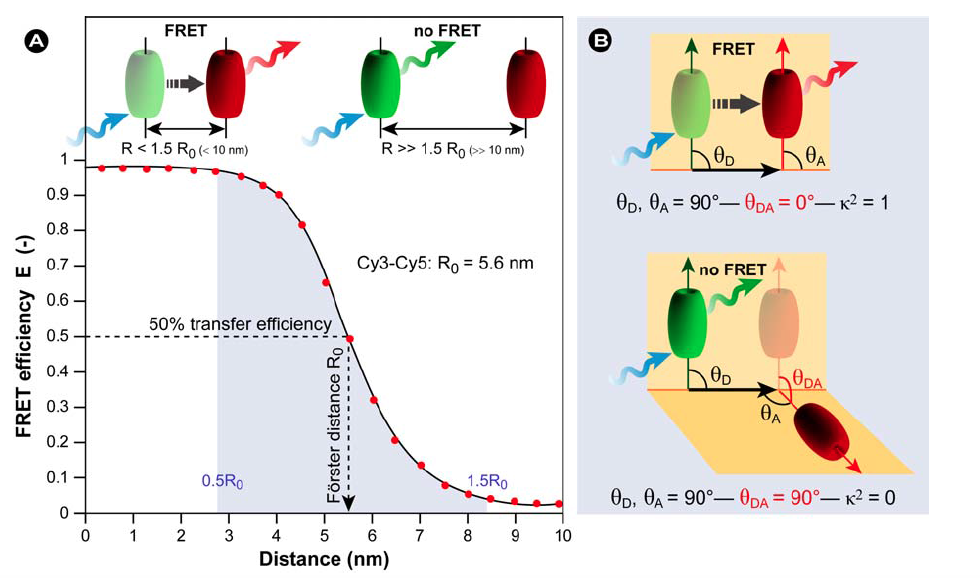
\includegraphics[width=0.9\textwidth]{nfm28}
\\* Эффективность фёрстеровского механизма переноса энергии

скорость передачи энергии $k_t = \tau_d^{-1}\left(\frac{R_0}{r}\right)^6$

$\tau_d$ - невозмущенное время жизни

$R_0$ - фёрстеровский радиус, его величина от 1 до 10 нм.

\end{center}
\column{5.5cm}
\begin{itemize}
\item На расстояниях много меньше длины волны излучательные механизмы передачи энергии невозможны.

\item Безызлучательные механизмы: \\*(1) электростатической природы (по Фёрстеру) на б\'ольших расстояниях \\* (2) обменной природы (по Декстеру) на максимально близких расстояниях.

\item Необходимо, чтобы спектр испускания донора перекрывался со спектром поглощения акцептора: например, родамин (акцептор), 590 нм, и флуоресцеин (донор), 458 нм.
\end{itemize}
\end{columns}

\end{frame}

\begin{frame}{Основа метода}
\begin{columns}[c]
\column{6.5cm}
\begin{center}
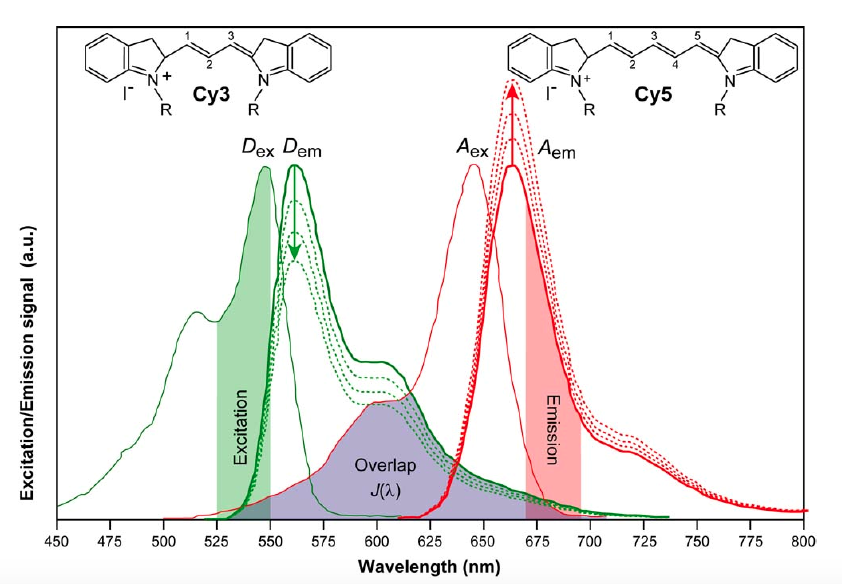
\includegraphics[width=0.9\textwidth]{nfm29}
\\* Достаточно перекрытия в 30$\%$
\end{center}

\begin{itemize}
\item \colorbox{yellow!30}{сенсибилизация флуоресценции} - излучает не тот объект, который мы возбудили, а другой, причем свойства этого излучения определяются характером передачи энергии, свойствами акцептора и окружающей среды

\end{itemize}

\column{6.5cm}
\begin{center}
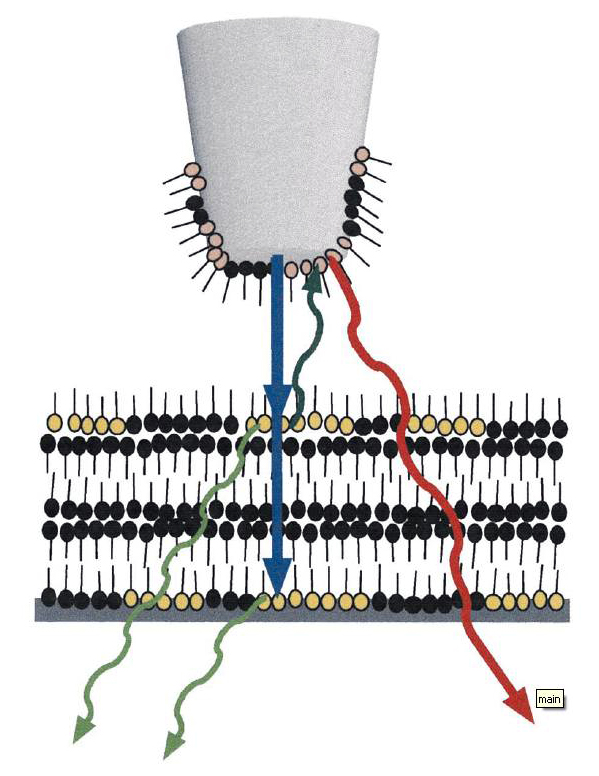
\includegraphics[width=0.9\textwidth]{nfm23}
\\* Зонд и образец покрываются пленками Ленгмюра-Блоджетт
\end{center}
\end{columns}

\end{frame}

\begin{frame}{Время разрешенная методика}

\begin{center}
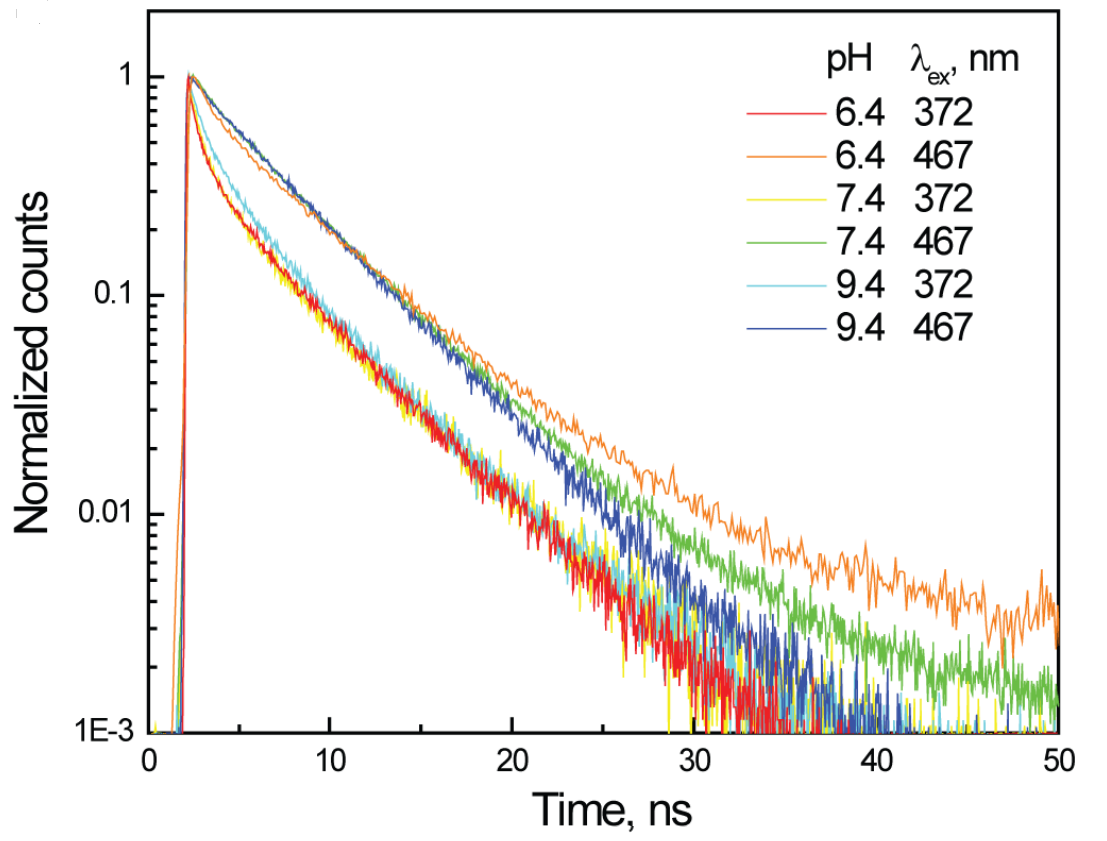
\includegraphics[width=0.8\textwidth]{nfm36}
\\* Так как флуоресценция - это процесс, протекающий во времени, это позволяет нам следить за динамикой (пример соверменного светопереключаемого белка WasCFP, синтезированного в группе Сергея Лукьянова, Sergey A. Lukyanov et al. Scientific Reports. 2012).
\end{center}

\end{frame}

\begin{frame}{Возможности метода}

\begin{center}
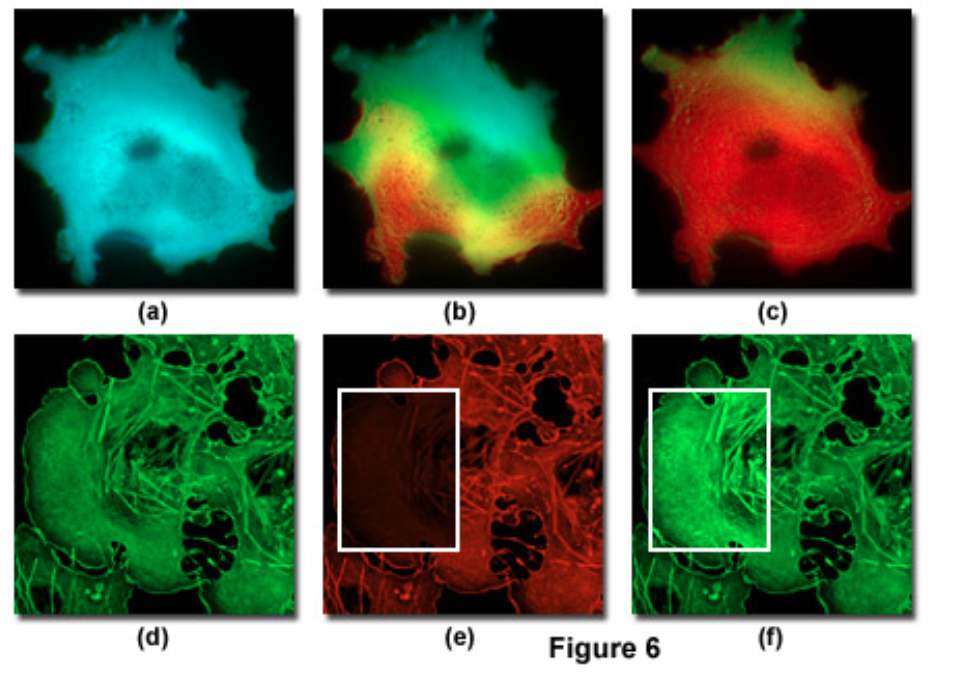
\includegraphics[width=0.8\textwidth]{fret_images}
\\*(a-c) \small{Динамика кальция в клетке карциномы человека}
\\* (d-g) \small{Клетки печени африканской обезьяны помещаются в раствор с холерным токсином, окрашенным донором (Cy3, зеленый) и акцептором (Cy5, красный). Видим, как фотообесцвечивание акцептора приводит к переходу донора от тушения к свечению.}
\end{center}
\end{frame}

\begin{frame}{Важные черты}
\begin{itemize}
\item Необходимо различать два термина \textcolor{red}{фотообесцвечивание (photobleaching)} и \textcolor{blue}{тушение (quenching)}. Первое представляет из себя необратимый процесс такой перестройки молекулы, когда на данной частоте она уже не может светить. Тушение -  процесс обратимый. Фотообесцвечивание акцептора приводит донора в состояние свечения \textcolor{red}{(dequenching)}.
\item FRET - это лишь один метод из семейства методов. Многие из них не являются ближнепольными. Например, FRAP - это fluorescence recovery after photobleaching.
\item Так как все упомянутые процессы протекают во времени, это позволяет создавать время разрешенные методы, т.н. time-lapse microscopy
\end{itemize}

FRET миркоскопия относится к классу \textcolor{blue}{s-SNOM}. Однако есть фарианты ближнепольной флуоресцентной микроскопии и в \textcolor{blue}{c-SNOM}. См. работы David Richards.

\end{frame}

\begin{frame}{Основа метода}
\begin{columns}[c]
\column{5.5cm}
\begin{center}
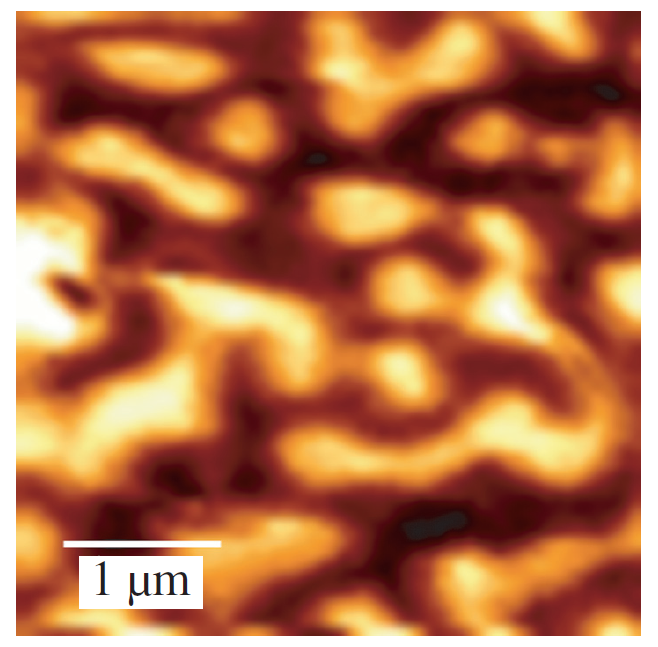
\includegraphics[width=0.8\textwidth]{nfm34}
\\* Смесь двух светоизлучающих полимеров, которая по мере выпаривания раствора, в котором они находятся, самоорганизутся на поверхности.
\end{center}

\column{7cm}
\begin{center}
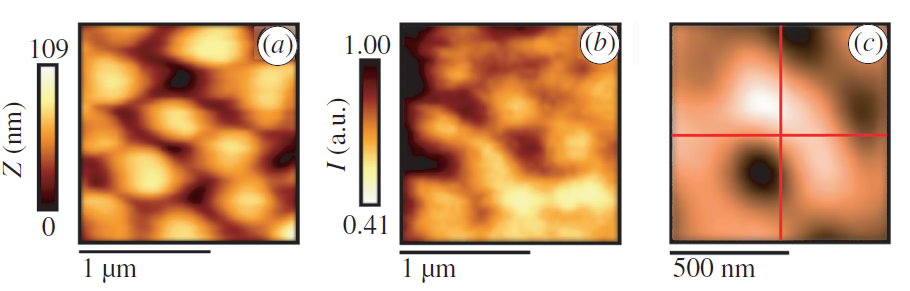
\includegraphics[width=0.9\textwidth]{nfm35}
\end{center}

В данном эксперименте бинарный раствор полимеров, которые используются в солнечных батареях (F8BT и PFO). Если мы используем длину волну 325 нм, возбуждающую только первый и затем рассмотрим корреляцию топографии, полученной на АСМ с картиной БП флуоресцеции, взятой с инвертированным контрастом, то можно увидеть, что области протрузии являются темными, то есть состоят из PFO. 

\end{columns}

\end{frame}

\plain{}{Оптические антенны на апертурных зондах}

\begin{frame}{Фото двух видов зондов}
\begin{columns}[c]
\column{6.5cm}
\begin{center}
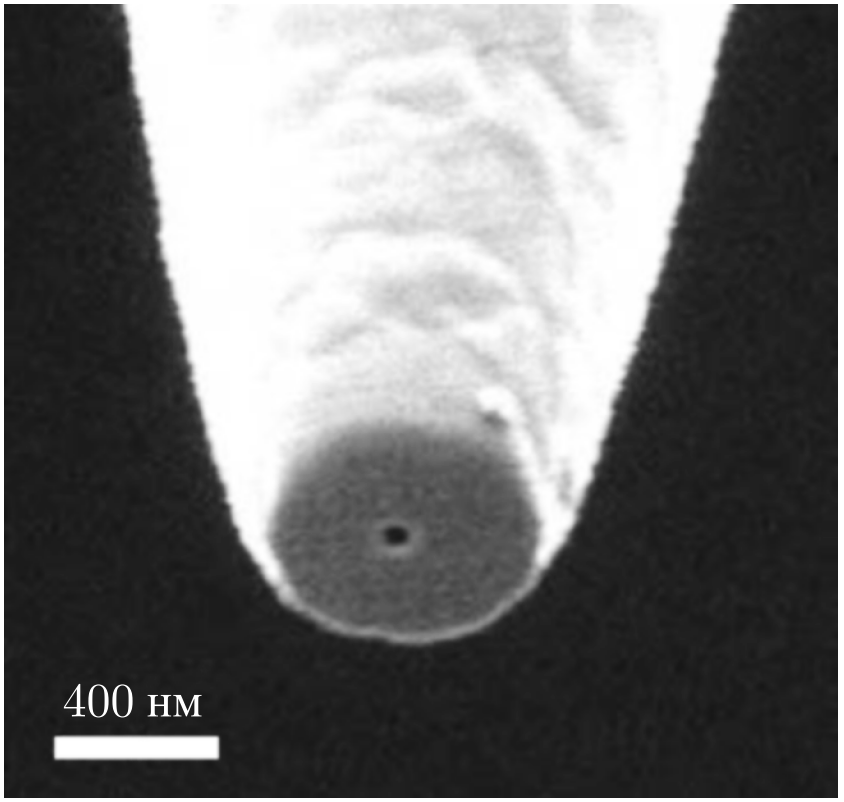
\includegraphics[width=0.8\textwidth]{nfm13}
\\* Апертурный зонд без дополнительной оптической антенны
\end{center}

\column{6.5cm}
\begin{center}
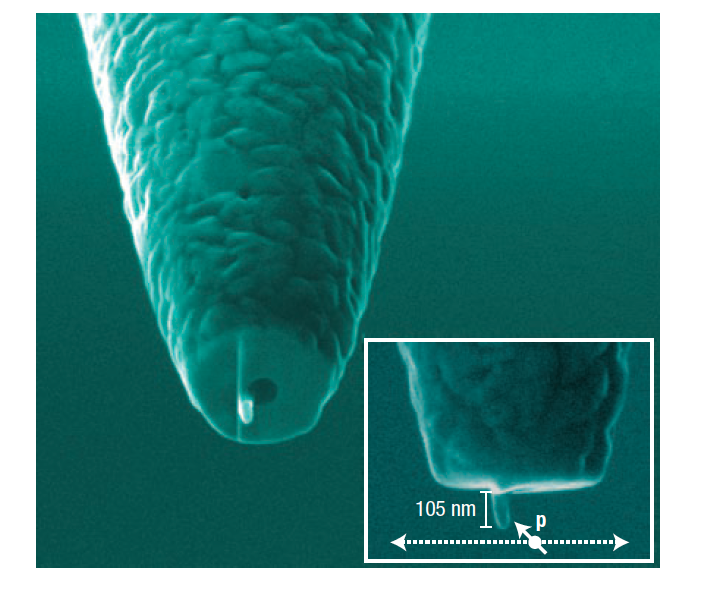
\includegraphics[width=0.9\textwidth]{nfm22}
\\* Апертурный зонд с протрузией, играющей роль оптической антенны
\end{center}
\end{columns}
В силу того, что, как мы говорили на первый лекциях, излучающий диполь имеет различную индикатриссу рассеяния в ближнем и дальнем поле, значит, его излучение также чувствительно к расстоянию. Этот факт становится еще одним инструментом исследования.

T.H. Taminiau et al. Nature. 2008.

\end{frame}

\begin{frame}{Промежуточные итоги:}

В классической оптике разрешение оптического прибора определялось только длиной волны излучения, которое используется для подсветки.

В ближнепольной микроскопии, количество параметров, которые определяют разрешающую способность и возрастает, 
\begin{itemize}
\item кроме длины волны излучения
\item это и форм-фактор оптической антенны (в качестве которой может выступать как сам зонд, так и специально организованная на его конце структура)
\item и ее восприимчивость
\item существенное влияние на разрешающую способность начинает оказывать и свойства ЭМ изучаемой среды и подложки
\item задача разделения дифракционно-ограниченного сигнала засветки и ближнепольного сигнала становится очень важной
\item необходимо учитывать множество причин для  артефактов, таких как несовершенство геометрии зонда, топографических и др.
\end{itemize}


Многие из этих обстоятельств могут быть обращены на пользу оптическому разрешению.



\end{frame}

\begin{frame}{Fourier Transform Infrared Microscopy}

Визуализация двух фаз пентацена, проникающих друг в друга

\begin{center}
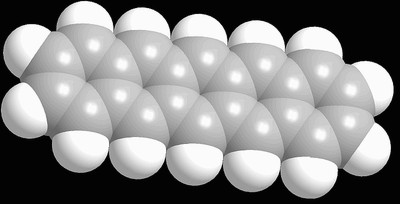
\includegraphics[width=0.8\textwidth]{pentacene}
\\Схема эксперимента по визуализации пентацена. Разрешающая способность 20 нм
\end{center}

    
\begin{center}
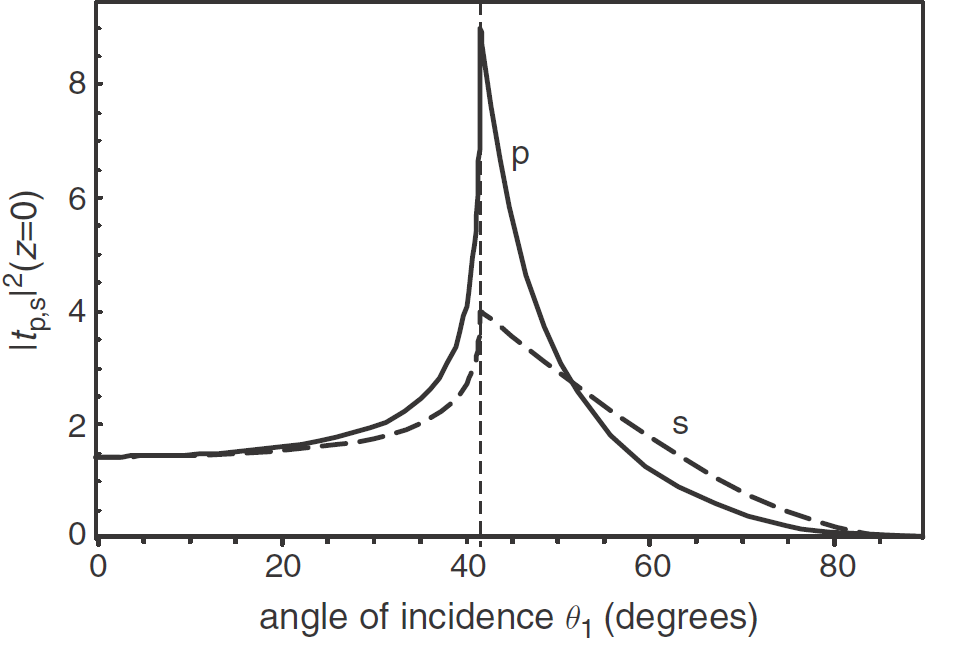
\includegraphics[width=0.8\textwidth]{ftir}
\\Схема эксперимента по визуализации пентацена. Разрешающая способность 20 нм
\end{center}
    
\end{frame}


\end{document}


